%\chapter{Collaborative tools}
\chapter{Introduction to Moodle and more command line skills: DRAFT VERSION}
\newcommand{\moodle}{\textsf{Moodle}}
\newcommand{\Moodle}{\textsf{Moodle}}

\minitoc

\notesurl{desktop2}

\begin{note}
  This is the fifth, two hour, lab.

  There was a feeling that the getting started with Moodle material might be a little light for a 2 hour session, so perhaps put some more Desktop oriented material in here as well.

  Has change of position (?) of this lab made any difference to how we tell students about first tutorial?

  Do we need some breakout boxes in this script?
  
  
  which supports COMP10120. You should also use this lab session to complete the \emph{Individual Learning Profile} questionnaire which is hosted inside \moodle.

\moodle\ is a \emph{Virtual Learning Environment} (VLE) that allows the classroom to extend onto the web.
  
\end{note}


\section{Getting started with \moodle}
\label{sec:introduction-moodle}

In this lab session you'll be introduced to the \moodle\ Virtual Learning Environment (VLE). \moodle\ is an Open Source platform designed to support face-to-face teaching by providing an online place to upload resources for course units. It also provides useful  tools such as discussion forums and quizzes. We use \moodle\ for several of our course units, which typically have a single `course unit site' within our \moodle\ environment.

%Why is Moodle being used for COMP10120
\moodle\ has several features which make it well suited to supporting this course-unit. These include:
\begin{itemize}
\item It's one useful way of communicating with your tutor and members of your tutor group 
\item It allows us to give each group a wiki which you'll use to collaboratively document your project work.
\item It provides a structure to help organise activities you should be doing on a week-by-week basis.
\end{itemize}

Log in to \moodle\ by pointing your web browser at: \urlnop{moodle.cs.man.ac.uk} and using your University credentials. 

After successfully logging into \moodle\ for the first time, you'll be presented with a form to complete the details of your \moodle\ profile. Add your first and last names; your email address; the city/town where you live (for most people this will be Manchester); and add a short description of yourself. Select the `Update profile' button to complete your \moodle\ registration. Assuming that worked okay, the next page to appear will be the \moodle\ home page (see  Figure~\ref{figure:moodle-home})

\begin{figure}
\centerline{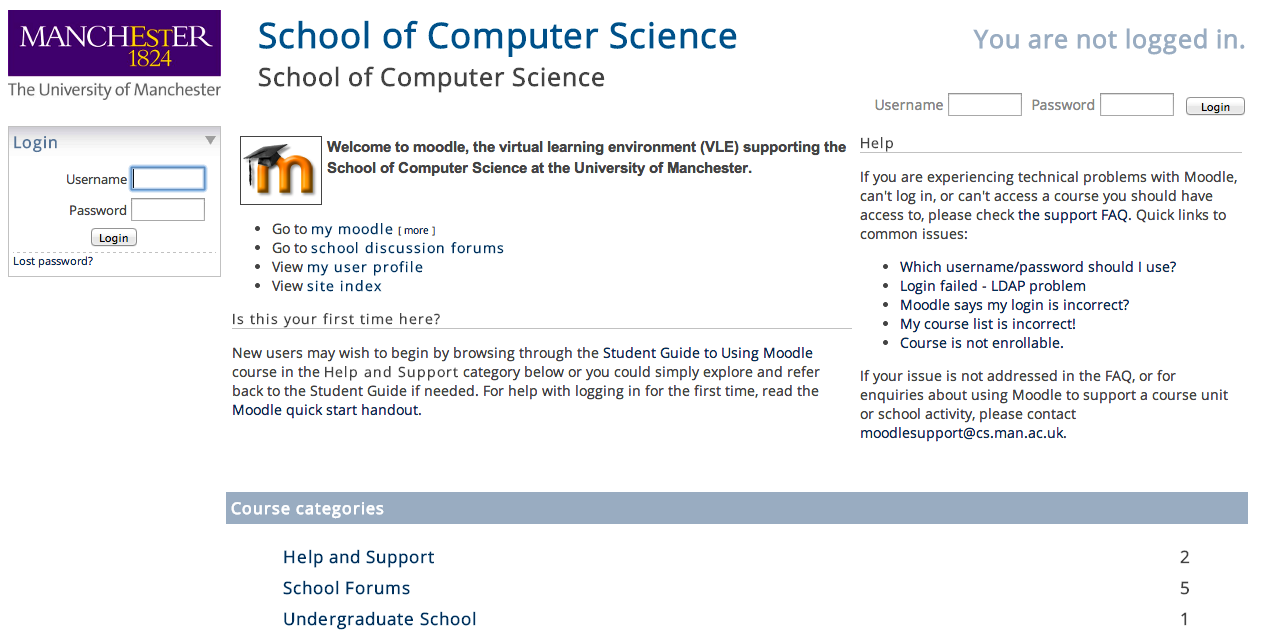
\includegraphics[width=15cm]{images/moodle-home}}
\caption{Moodle Home Page}\label{figure:moodle-home}
\end{figure}

Take a few minutes to browse though the \emph{Getting started with \Moodle} guide which is deliberately located outside the \moodle\ environment so that you can get at it in case you're having problems with \moodle\ itself. You can find it at: \urlnop{octette.cs.man.ac.uk/moodleintro} (see Figure~\ref{figure:moodle-start}).

\begin{figure}
\centerline{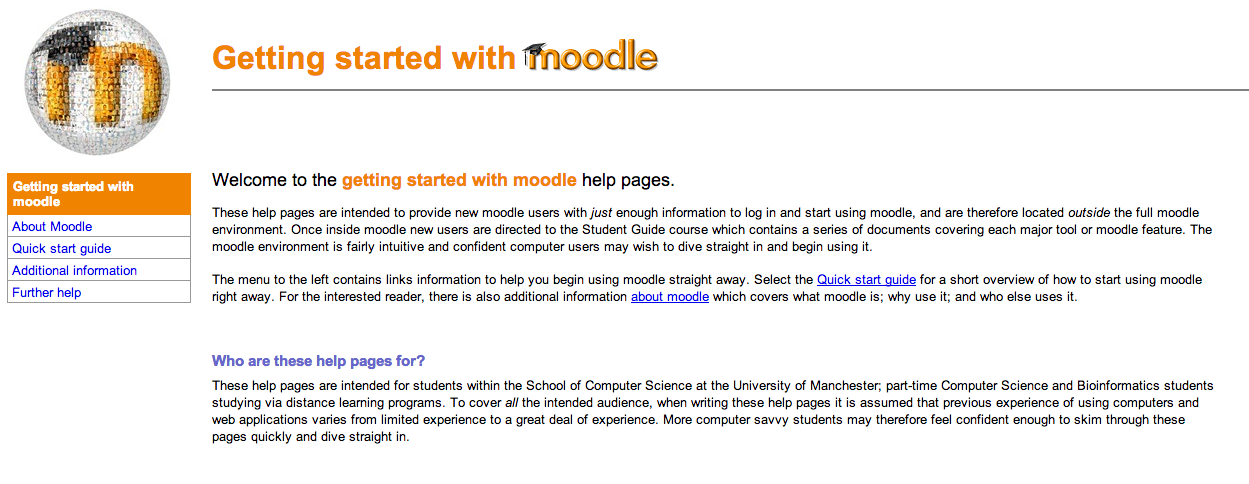
\includegraphics[width=15cm]{images/start-moodle-page}}
\caption{Getting started with Moodle}\label{figure:moodle-start}
\end{figure}

\subsubsection*{Brief overview of the \moodle\ home page}
\label{sec:brief-overv-moodle}


The \moodle\ home page lists several categories in which \moodle\ course unit sites are organised (make sure you scroll down to see them all). \moodle\ course unit sites exist for many, but not all, course units within your degree programme. There are also a number of \moodle\ sites that provide support to staff and students in other ways, such as a general CS help sites and the Staff Student Consultative Committee public site.

You can find links to sites by either locating the link in the appropriate category, for example look in \emph{Undergraduate School/First Year} for COMP10120; or you can enter \emph{COMP10120} into the \emph{Search courses} field at the bottom of the course list and select the course unit title from the search result(s).

Other things to look out for on the front page include the link to your \moodle\ user profile and the link to the \emph{my moodle} feature. We'll come back to these later on.


%Your turn


Make sure you can find the COMP10120 course unit site and are able to access it. To get back to the \emph{\moodle\ home page} you should click on the \moodle\ link in the navigation bar underneath the course unit title at the top of the page. This is always the first element in the link trail. If you navigate further into the course unit site, to return to the \emph{course unit site front page} just click on the COMP10120 link in the navigation bar. This is always the second element in the link trail.

Now locate the course titled \emph{Student Guide to Using Moodle} (in the category \emph{Help and Support}). Have a browse through what help material is provided here. You may wish to revisit this site to learn how to use one of the \moodle\ activities or understand one of \Moodle's features.

\subsection{The COMP10120 course unit site}
\label{sec:comp10120-course-uni}


If you haven't already, navigate to the COMP10120 site and start to look at how the site is structured and what tools have been provided (see Figure~\ref{figure:101-moodle-page}).
Things you should note about the structure of the site:

\begin{figure}
\centerline{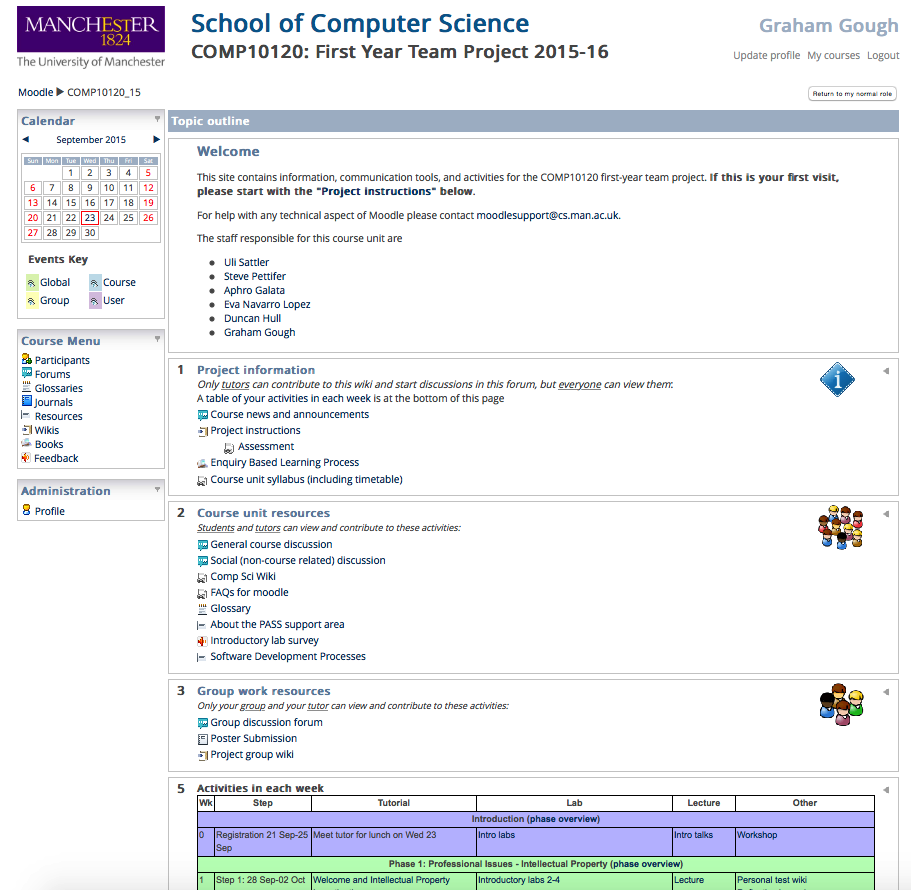
\includegraphics[width=15cm]{images/101-moodle-page}}
\caption{COMP10120 Moodle Home Page}\label{figure:101-moodle-page}
\end{figure}


\begin{itemize}
\item 
All instructions for the course unit are located in the \emph{Project information} area towards the top of the site. Take a look at each of the links in this area. In particular, familiarise yourself with the front page of the \emph{Project instructions} and read at least the \emph{Introduction to the tasks and activities} (and then click through to the \emph{Phases and Tutorials} page to get an idea of the course unit structure).

\item Back on the course unit site, the next section is called \emph{Course unit resources}. If you have a query about the course unit, please use link to the \emph{General Course Discussion Forum}.

\item The next section is called \emph{Group work resources}. This is your tutor group's area and should be used to communicate with members of your team (by using the forum) and to document your work (in the wiki).

\item Finally, the bottom of the course unit site has a table of all your activities for this course-unit. The different phases are colour-coded to help you spot the one you want. The row for each week contains links to information about what you should be doing in that week and tools/resources applicable to the week. (Don't forget to read the \emph{phase overview} first.)

  The \emph{Other}  column includes resources for your personal use, that you are expected to complete over the course of the year. In particular you should note the \emph{reflective journals} for each week of the first semester. You are expected to reflect on the questions detailed inside the journal each week.
\end{itemize}

% The remaining instructions for this lab session can be found
% directly within \moodle\ itself. Click on \emph{Introduction to \Moodle} % in the \emph{Lab} column for \emph{Step 1} in the green (\emph{Phase 1}  section.

\subsection{Lab deliverables}
\label{sec:lab-deliverables}

\begin{note}
  Do we want a list of deliverables for each lab? Should they be at the start of the script?
\end{note}

By the end of this lab session, ensure you have completed the following tasks.

\begin{itemize}
\item 
Posted a welcoming message to your tutor group (see Using forums below).

\item Create your set of practise wiki pages (see Using wikis below).

\item Completed the Individual Learning Profile questionnaire
\end{itemize}

There are also a number of optional tasks you should aim to complete if you have time during the lab.

\subsection{Using forums}
\label{sec:using-forums}


Most of you will have used discussion forums in some way or another, whether on your favourite social networking site or on some other website. \Moodle's forums aren't too different to any other, however, you should note a few things:

Most forums are configured so that copies of each posting will be emailed to other course unit members. In a group forum, copies are only emailed to other group members; in a course forum copies are emailed to everyone.

In most cases you will have the option to remove your subscription to such emails. Please don't do this, at least not at the moment.

In your user profile you have the option to receive \moodle\ emails as a single daily digest rather than as multiple emails each day; if you're finding you're getting a lot of email from \moodle\ this might be a sensible option to select (but keep it mind that you'll lose some of the immediacy of receiving individual emails). 

You might not be able to post messages in all forums. Some forums (e.g. course announcement forums) will only allow tutors to start new topics of discussion, but will allow students to reply to those topics once started.

%Your turn
Visit your Group discussion forum on the COMP10120 site and click on \emph{Add a new discussion topic}  to begin a new discussion thread. Write a short forum posting to introduce you to your other group members and your tutor. Let them know where you are from, tell them a little bit about yourself. Warning: the current in-line HTML in \moodle\ can sometimes misbehave, especially if you try to apply lots of formatting. Therefore concentrate on content rather than presentation.

Note that your discussion posting won't be emailed to the other members of your group until about 30 minutes after you submit the posting. This is to allow time for you to edit it in case you spot a mistake.

If you want to find out more about using discussion forums, look through the \emph{How to use the forums}  help book in the \emph{Student Guide to Using \Moodle} course. There is also a help book called \emph{Using \moodle's HTML editor} which you may also find useful.

\subsection{Using wikis}
\label{sec:using-wikis}


You have almost certainly come across wikis before, and will no doubt have looked things up in \wikipedia{Wikipedia}{Wikipedia}, the world's biggest wiki, many times. Unlike many other online collaboration systems which constrain users in various ways by pre-determining the type of content that can be create (for example sites like Instagram and Flickr are designed for sharing photographs, where as Soundcloud is for sharing audio), and also categorising users as having different types of access (e.g. administrators, moderators, regular users and so forth), the technology behind wikis typically takes a very liberal approach to both users and content. They generally allow any user to make any kind of change to any kind of content, and rely on \textit{social} conventions established by the community to keep things sane. In particular, every edit, deletion and addition to the wiki is stored, providing a complete history of wiki changes. Old versions of pages and be retrieved and compared to new versions of pages. Wikis are typically edited using a simple mark-up syntax where the focus is on content rather than fancy presentation.


As well as creating sites like Wikipedia, wikis are frequently used by software development teams to document their project. The ability to look back to previous versions of documents and the for multiple authors to collaborate on producing the documentation without having to worry too much about `process' is particularly useful in such environments.

During COMP10120 you'll required to document many aspects of your work using a group wiki provided by \Moodle. \Moodle's wiki isn't as powerful as others you may have come across as it is primarily tailored towards teaching, but it does allow you to use \Moodle's standard in-line HTML editor to help you with formatting.

%Your turn
In the bottom \emph{Resources for individual use} section of the COMP10120 site you will find a link to a wiki called \emph{Personal test wiki} which is private for you and you only. It is provided to allow you to practise how to use \moodle\ wiki syntax before you start using your shared group wiki. If you have used a wiki before then you may find \Moodle's wiki syntax is slightly different to that which you are used to.

For this short exercise you will need to read through some of the help documentation hosted inside \moodle. In a new window or tab navigate to \urlnop{moodle.cs.man.ac.uk} again and enter the \emph{ \emph{Welcome to the Student Guide to Using \Moodle} }course in the \moodle\ \emph{Help and Support}  category (you may be asked to 'enrol' on this course, just select 'Yes'). Scroll down to the section about Wikis and select the \emph{How to use the wiki tool} book.

The aim of this short exercise is to create a simple wiki page with two or three wiki links to other pages; incorporate an image; and attach and link to a binary (non-image) file. It is important that you follow this mini-tutorial through to the end as it will ensure you know how to do all the basic tasks needed to help build your own group wiki during the project.

For the purposes of this mini-tutorial you are asked to create a small wiki about yourself.

Start by opening your Personal test wiki. You will be presented with the \moodle\ editor which won't contain any content yet. Enter a title for the page, something like \emph{About Me} will do.

Select the \emph{Save} button. You should now see the first page of your wiki with the content you just added. Now select the \emph{Edit} tab so that you can add more content.

Create a short bullet list containing the items \emph{My hobbies},  \emph{My music}  and \emph{My files}  Save the page again and check the results, then select the Edit tab again. Now turn the three items into wiki links. To do this, just put a single set of square brackets around each of the terms, like this: \emph{[My hobbies]}  \emph{[My music]}  \emph{[My files]}  Save the page again and look at what just happened. If everything worked correctly each term enclosed in square brackets should now look like this: term? (emboldened text followed by a hyperlinked question mark).

Select the question mark symbol on the \emph{My hobbies} term. Note this opens up a new wiki page called \emph{My hobbies} for you to populate with content. Add some text to describe a few things about what you like to do with your time and then select Save.

This is the basic process by which you build up a wiki into a series of linked pages. Note that at the bottom of the page you just created is a list of \emph{Referring links}  This means \emph{a list of pages that link to this one}  Select the link back to the front page.

In the Student Guide to Using \moodle\ course look at the help book on wikis and read the chapter titled \emph{Unique names for pages}  in particular instructions on how to make the link text different from the linked page name. Now go back and change your first wiki page so that the link to the page \emph{My hobbies} contains the link text \emph{My interests} (but still points to My hobbies). Your list should now contain the items \emph{My interests},  \emph{My music}  and \emph{My files} 

Now go back and select the question mark link for the \emph{My music} link and add some content to this page too. You could write about music you love (or music you hate!).

In the last part of this mini-tutorial, you will need to add a small picture to your wiki and a small file. First we need some files to play with. If you have a small picture that you took yourself, great, you own the copyright on it. Create a small text file using any text editor containing any text you like. If you don't have a picture to use and can not source a copyright free image, you will find a link to an example image in the summary text box of the wiki above the first page. There is also a link to a sample text file there too.

In the Student Guide to Using \moodle\ course look at the help book on wikis and read the chapters titled \emph{Attaching binary files} and \emph{Linking to attached files}  From your wiki's front page select the question mark link for the \emph{My files} link to create its page content. Attach your text file to the page from the wiki's Attachments tab as described in the \emph{Attaching binary files} chapter of the help book. Then return to the edit tab and add the following text:

\emph{Wikis allow users to attach files, such as this one here}  

Turn the word \emph{here} into a link to the text file you just uploaded following the instructions in the \emph{Linking to attached files} chapter of the help book.

Carefully read the chapter of the help book titled \emph{Incorporating images}  Now add the following text and add the image you grabbed earlier below the text.

\emph{Wikis also allow users to incorporate images such as this one.} 

Experiment with changing the alignment of the image as described in the help book.

Finally, browse through the remaining documentation in the Wiki help book so that you have an overview of what other information is there and can refer back to it in the future if needed. If you have any questions about how to use the wiki tool, post a message to the General course unit discussion forum.

\subsection{Individual Learning Profile questionnaire}
\label{sec:indiv-learn-prof}

Before the end of the lab session make sure you complete the \emph{Individual Learning Profile questionnaire}. You will find it in the \emph{Resources for your individual use} section at the bottom of the \moodle\ course unit site. This activity is to help you to reflect so that you can understand your own basic skills and abilities required for your academic life. It may also be looked at by your personal tutor so the School can be better placed to address your particular needs during your time in the School of Computer Science. This information will only be visible to you, to your tutor and to the course unit organisers.

\subsubsection*{Writing your journal}
\label{sec:writing-your-journal}


One of the aims of this course unit is to encourage you to develop the habit of thinking about the way you are learning and working, and trying to identify ways in which these could be improved. The process of reflection is key to this, but is not something that comes naturally to many of us. In most week slots of the course unit site you will find an instance of the Journal activity. The summary text of each journal contains prompts to aid your reflection that week. The journal is very simple \moodle\ tool which provides you with an editable text area supported by \moodle\ HTML editor. Selecting the \emph{Start or edit my journal entry} button opens your journal. Any entries you put into your journal will be completely private to you and your personal course unit tutor. A limited number of the course unit organisers have access to all students journals, but will respect your privacy and will not be looking at them.

At some time towards the end of this week, start your journal entry for the current week and post your answers the prompts provided.

\subsection{What else is on \moodle?}
\label{sec:what-else-moodle}


As well as course unit sites for many of your course units, there are also a number of open areas within \moodle. Within the \emph{Support Forums} category you will find a number of sites where you can seek help about specific areas within computer science, e.g. the C / C++? Programmer's Forum. The \emph{Student / Staff Groups} category includes a site where you can post up questions or topics of discussion for the Staff Student Consultative Committee. All these open courses are indicated by the guest user icon (a small person icon or a side-on face depending on your chosen \moodle\ theme). Have an explore and see what is there. More open site are likely to be added over the year.

\subsection*{Playing and personalising}
\label{sec:play-pers}


If you have time left in the lab session, spend some time personalising your \moodle\ account. Things you could do include:

Uploading a small photo or image to represent yourself to your \moodle\ profile.

%Personalising your my \moodle\ area.

Take a closer look at the advanced options in your \moodle\ profile and investigate what they do (read up about this in the \moodle\ help course books first).


 Look ahead on the COMP10120 site to get a feel for what you will be doing over the coming year.


\section{More command line skills}
\newcommand{\cmdname}[1]{\cmnd{#1}{#1}}
\newcommand{\ilinput}[1]{\ttout{#1}}
\newcommand{\crsname}{COMP10120}
\newcommand{\Dcrsname}{???}
\newcommand{\crsnamelc}{comp10120}
\newcommand{\return}{\relax}

This section to practice your command line skills and prepare for next week

\subsection{Creating a directory structure}

You're now going to use the \cmdname{mkdir} (``make directory'') command
to create some directories. Type

\begin{ttoutenv}
  mkdir \crsname\return
\end{ttoutenv}
%
Check that this directory has indeed appeared using \cmdname{ls}.

It's important that directories we ask you to make for your work have
exactly the names we specify. Unix will let you use any names you
like, but we have to impose conventions for administrative reasons.

If you made a mistake, e.g. \fname{\crsnamelc} instead of \fname{\crsname},
you can remove the directory while it is still empty with the
\cmdname{rmdir} command: e.g.
%
\begin{ttoutenv}
  rmdir \crsnamelc\return
\end{ttoutenv}
%
And then try to make it correctly.

The \cmdname{cd} (``change directory'') command allows you to move around
the tree by changing your current working directory. Type
%
\begin{ttoutenv}
  cd \crsname\return
\end{ttoutenv}
%
to make \crsname{} your working directory. Check that you have changed
current directory using \cmnd{pwd}{pwd}.

  
Now make directories for each of the \crsname{} exercises.

\begin{ttoutenv}
  mkdir ex1 ex2 ex3 \return
\end{ttoutenv}
%  mkdir ex1 ex2 ex3 ex4 \return
%
Recall that the \cmdname{cd} command on its own takes you back to your home
directory, wherever you may be when you invoke it.  Try this out by
typing

\begin{ttoutenv}
  cd \return
\end{ttoutenv}

Check that you are now in your home directory.

Your directory structure should now look something like this
%\begin{firstonly}
     \begin{center}
       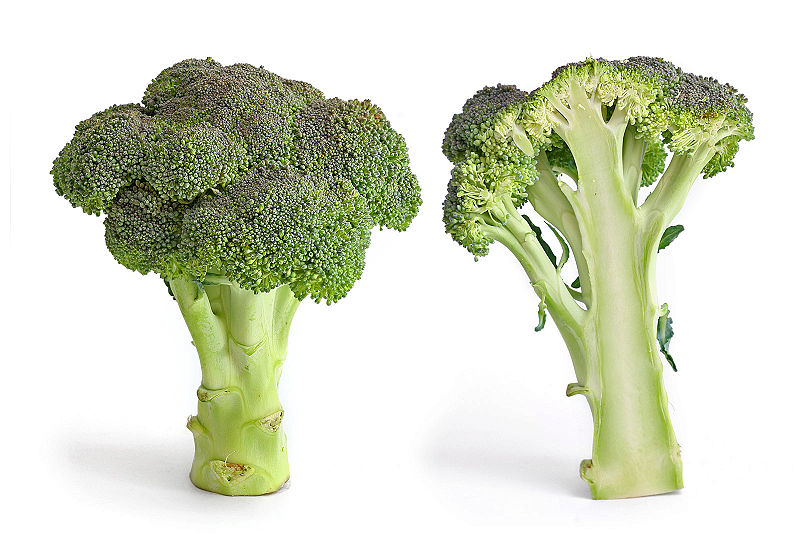
\includegraphics[width=0.4\textwidth]{images/broccoli} %ps/dirs.eps}
     \end{center}
%\end{firstonly}

%\begin{msconly}
%     \begin{center}
%       \includegraphics[width=0.4\textwidth]{ps/dirs-msc.eps}
%     \end{center}
%\end{msconly}
     
The easiest way to check this is to use (from your home directory)
\cmdname{ls} with the \ttout{-R} flag. This shows the whole tree
below your current working directory (\ttout{-R} is short for
\wikipedia{Recursion}{``recursively'}'  -- look up the word in a dictionary, or wait until later for a
 definition!).

\begin{ttoutenv}
\$ ls -R 
\end{ttoutenv}
%

  Now you should make a directory for the COMP16121 course unit
  %(or COMP16920
  %if you
%  are an ABIS student) with
  %are a CSE student)
  with
  sub-directories for each of the 10 exercises associated with that
  course. You \emph{must} use the same convention as above:
  capital ``COMP16121'' and lower case ``ex1'', etc..

You must get your directory structure right before continuing -- ask a
member of the lab staff to check it at this point.


\subsection{Copying, moving, and removing files}

This subsection re-introduces three commands used for copying, moving and
removing files. We first describe each command and then invite you to
practice using them.

\noindent The \cmdname{cp} (copy) command has two forms.

\begin{note}
  fix <file> [file] notation
\end{note}

The first general form is
\begin{ttoutenv}
  cp <file> <file> \return
\end{ttoutenv}

For example

\begin{ttoutenv}
  cp file1 file2 \return
\end{ttoutenv}
%
makes a copy of the file \fname{file1} and calls it \fname{file2}.  If
a file called file2 already exists, \emph{the existing \fname{file2} will be  overwritten
with a copy of \fname{file1} and lost without warning}.

The second form is slightly different:
\begin{ttoutenv}
  cp <file(s)> <directory>
\end{ttoutenv}
%
For example

\begin{ttoutenv}
  cp file1 file2 file3 dirname \return
\end{ttoutenv}

This copies the files \fname{file1}, \fname{file2}, \fname{file3} into
the directory \fname{dirname}, again overwriting any files already
there with the same names.

The command \cmdname{rm} (remove) is used to delete files.
\begin{ttoutenv}
  rm <file(s)>
\end{ttoutenv}
%
throws away the specified files -- always take great care when using
\cmdname{rm}, it is not reversible.

The \cmdname{mv} (move) command is similar to \cmdname{cp}, but it just moves
the files rather than makes copies. Again we have the two forms
\begin{ttoutenv}
  mv <file1> <file2> \return
\end{ttoutenv}
and
\begin{ttoutenv}
  mv <file(s)> <directory> \return
\end{ttoutenv}

The effect is like a copying followed by removing the sources of the copy,
except it is more efficient than that (most of the time).
For example
\begin{ttoutenv}
  mv file1 file2 \return
\end{ttoutenv}
is like doing
\begin{ttoutenv}
  cp file1 file2 \return
  rm file1
\end{ttoutenv}
and
\begin{ttoutenv}
  mv file1 file2 file3 dirname \return
\end{ttoutenv}
is like doing
\begin{ttoutenv}
  cp file1 file2 file3 dirname \return
  rm file1 file2 file3
\end{ttoutenv}

Before continuing, answer this question and check your answer with a
member of staff: how do you \emph{rename} a file in Unix? Don't guess -- you
know the answer, unless you are going too fast.

Now for some practice. Go to your home directory
%
\begin{ttoutenv}
  cd \return
\end{ttoutenv}
%
and copy the file called \fname{lightbulbs} in the \fname{\Dcrsname}
directory to your current working directory:

\begin{note}
Tell them about .  
\end{note}

\begin{ttoutenv}
  cp \Dcrsname/lightbulbs .  \return
\end{ttoutenv}
%
Note that \ilinput{\Dcrsname} must be in uppercase and the full stop is
essential.  If you now do an \cmdname{ls}, you should see that the
file called \fname{lightbulbs} has appeared in your directory:

\begin{ttoutenv}
  ls \return
\end{ttoutenv}

If no file called \fname{lightbulbs} has appeared, the following will
probably provide an explanation. If it did appear, read this anyway, just to
check that you understand what you did right!

The \cmdname{cp} command needs two arguments. In this case, the file
you are copying is \fname{\Dcrsname/lightbulbs}, and the directory
you are copying it to is ``.'' (that is, your current working
directory -- remember every directory has a reference to itself within
it, called `.'?). If you missed out the dot, or mis-spelt
\fname{\Dcrsname/lightbulbs}, or missed out one of the spaces, it
won't have worked. In particular, you may well have got a
``friendly'', helpful error message like:
%
%  Usage: cp [-ip] f1 f2; or: cp [-irp] f1 ... fn d2
\begin{ttoutenv}
  cp: missing destination file
  Try `cp --help' for more information.
\end{ttoutenv}
%
or
\begin{ttoutenv}
  cp: /opt/info/courses/\crsname/lightblurbs: No such file or directory
\end{ttoutenv}
or
\begin{ttoutenv}
  cp: \crsname/lightbulbs: No such file or directory
\end{ttoutenv}
%
If you get the first message, it means you used the command with the
wrong number of arguments, and nothing will have happened.
The others are examples of what you might see if you mistype the first
argument. If you do get an error message you need to give the command again,
correctly, to copy the lightbulbs file across.

So you now have a copy of the file, but, it's in your home directory.
You'll have to get into the habit of \emph{not} having all your files
in your home directory, otherwise you will quickly have an enormous list
that will take you ages to find anything in. The use of subdirectories
provides a solution to this problem, which is why you created some
earlier. Moving this file to the ``correct'' place gives you a chance
to practice the \cmdname{mv} command.

Move the file \fname{lightbulbs} to your \fname{\crsname/ex2} directory.

Notice that \fname{\crsname} is \emph{your\/} \crsname{} directory, while
\fname{\Dcrsname} is (an abbreviation for) \emph{our\/} \crsname{}
directory, from which you can read things but cannot write to.

Now go to your \fname{\crsname/ex2} directory and check that the file
has arrived there.

To make sure you understand \cmdname{cp}, \cmdname{mv}, and
\cmdname{rm}, go through the following sequence (in your
\fname{\crsname/ex2} directory), checking the result by looking at the
output from \cmdname{ls} at each stage

\begin{ttoutenv}
  cp lightbulbs bulb1 \return
  ls \return
  cp lightbulbs bulb2 \return
  ls \return
  mv bulb1 bulb3 \return
  ls \return
  cp bulb3 bulb4 \return
  ls \return
  rm bulb2 \return
  ls \return
  rm bulb1 \return
  ls \return
\end{ttoutenv}
Why does \ilinput{rm bulb1} behave differently to \ilinput{rm bulb2}?

\subsection{Wild cards}
An asterisk in a filename is a \textbf{wild card} which matches any sequence of
zero or more characters, so for instance, if you were to type (don't
actually do it!)
%
\begin{ttoutenv}
  rm *fred*\return
\end{ttoutenv}
%
then all files in the current directory whose names contain the string
``fred'' would be removed.

Try the effect of
%
\begin{ttoutenv}
  ls bulb*\return
\end{ttoutenv}
%
and
%
\begin{ttoutenv}
  ls *bulb*\return
\end{ttoutenv}

Now try
%
\begin{ttoutenv}
  echo *bulb*\return
\end{ttoutenv}
%
Are you surprised by the result?

One exception to the above rule is provided by the dotfiles; i.e. those
whose names begin with ``.''. The asterisk will not match a
``.'' at the start of a file name. To see what this means try the
following
\begin{ttoutenv}
  cd \return 
  ls *xinit* \return
\end{ttoutenv}
%
and
%
\begin{ttoutenv}
  ls .*xinit*\return
\end{ttoutenv}
and see the different output.

\subsection{Quotas}
The command

\begin{ttoutenv}
  quota\return
\end{ttoutenv}

shows you what your file store quota is, and how much of it you are
actually using. This is only of academic interest now, but may become
very important later in the year! You may find that you are unable to
save files, or even receive mail, if you use more than your quota of
file store. It is important that, if this happens, you do something
about it immediately.
%Some tips as to what do if this happens can be
%found on the \htmladdnormallink{local Software Links web
%%  page}{http://www.cs.manchester.ac.uk/software/}.
%  page}{\localSoftware}.

 
\subsection{Putting commands together}
Before you forget that you're in your home directory, change directory back to
your \crsname/ex2.

One of the simplest (and most useful) of Unix commands is
\cmdname{cat}. This command has many uses, one of which is to
con\textbf{cat}enate a list of files given as arguments and display
their contents on the screen. For example
\begin{ttoutenv}
cat file1 file2 file3 \return
\end{ttoutenv}
would display the contents of the three files \fname{file1},
\fname{file2} and \fname{file3}.
The output from \cmdname{cat} goes to what is known as the
\textbf{standard output} (in this case the screen).

If you type  
\begin{ttoutenv}
cat \return
\end{ttoutenv}
nothing will happen because you haven't given a file to \cmdname{cat}.
When run like this, it takes its data from the \textbf{standard input},
which in this case is the keyboard, and copies it to the standard
output. Anything that you now type will be taken as input by
\cmdname{cat}, and will be output once each line of the input is
complete. In Unix, end of input is signalled by \ilinput{<Ctrl>d}.
(Recall that typing \ilinput{<Ctrl>d} in your login shell will log you
out -- you have told the shell to expect no more input.) So, after
typing \cmdname{cat} above, if you type (we will omit the \return's
from now on, we hope you've got the message)
\begin{ttoutenv}
This is
some 
text for cat to 
digest
<Ctrl>d
\end{ttoutenv}
you will see the input replicated on the output (interleaved line by
line with the input). The first copy is the echo of what you typed as
you typed it, the second copy is output from \cmdname{cat}. This may
not seem very useful, and you wouldn't actually use it just like that,
%(An example where you really would have cat do just this is a bit too
%complicated to show here!) 
%We've merely asked you to do that to
but it illustrates the point that \cmdname{cat} takes its input and copies it
to its output. Using this basic idea we can do various things to
change where the input comes from and where the output goes.

\begin{ttoutenv}
cat > fred1
\end{ttoutenv}
will cause the standard output to be directed to the file \fname{fred1}
in the working directory (the input still comes from the keyboard and
will need a \ilinput{<Ctrl>d} to terminate it. Try creating a file
\cmdname{fred1} using this technique, and then check its contents.

\begin{ttoutenv}
cat < fred1 
\end{ttoutenv}
will take the standard input from the file \fname{fred1}
in the working directory and make it appear on the screen. This has
exactly the same effect as 
\begin{ttoutenv}
cat fred1 
\end{ttoutenv}

You can, of course, use < and > together, as in
\begin{ttoutenv}
cat < fred1 > fred2
\end{ttoutenv}
which will copy the contents of the first file to the second. Try this and
check the results.

We can, of course, do this type of redirection with other
commands. For example, if we want to save the result of listing a
directory's contents into a file we just type something like
\begin{ttoutenv}
ls -l > fred1
\end{ttoutenv}
(this overwrites the previous contents of \fname{fred1} without
warning, so be careful of this kind of use).

One of the other things that \cmdname{cat} can do is to put line
numbers on its output. It does this if you use the \ilinput{-n}
flag. Try
\begin{ttoutenv}
cat -n fred1
\end{ttoutenv}
Now suppose, for the sake of argument, we wanted to have a listing of the
names of the
files in the current directory, with each line numbered, and the result
saved in a file \cmdname{fred3}. You have just been given all the
information you need to do this -- so, how would you do it? Do it now.

Unless you've met Unix before, you probably did something like this
\begin{ttoutenv}
ls > tmpfile 
cat -n tmpfile > fred3
\end{ttoutenv}
Or if you didn't then try it now and examine the contents of
\fname{fred3}. The file \fname{tmpfile} can now be thrown away using
\ilinput{rm tmpfile}.

It's a shame we had to use an extra, temporary, file. Could we avoid
having to? Why do you think the following would not work?
\begin{ttoutenv}
ls > fred3 
cat -n fred3 > fred3
\end{ttoutenv}

A better way of doing the task, which avoids the use of a temporary file
is by use of a powerful Unix feature called the \textbf{pipe}. We just type
\begin{ttoutenv}
ls | cat -n > fred3
\end{ttoutenv}
The \textbf{pipe} symbol \verb+|+ indicates that the \textbf{standard
output} of the first command is to be \textbf{piped} into the
\textbf{standard input} of the second command, so no intermediate file
is needed.

We can construct another (slightly artificial) pipeline example using
just \cmdname{cat}.

\begin{ttoutenv}
cat < fred1 | cat > fred2
\end{ttoutenv}
The first \cmdname{cat} takes its input from
\fname{fred1} and sends its output into the pipe. The second
\cmdname{cat} takes its input from the pipe (i.e. the output from the
first \cmdname{cat}) and sends its output to \cmdname{fred2}. (How many
other ways can you think of to do this?)  This isn't a frightfully sensible
thing to do, but it does illustrate the principle of piping (long
pipelines of commands may be constructed), and more realistic examples
will appear in the exercises.

Standard output sent to the screen may come so fast that it
disappears off the top before you have had a chance to read it.
There are three ways around this problem.
\begin{itemize}
\item Using foresight, pipe the output into the command \cmdname{more}
  or \cmdname{less}
  which arranges to stop after each page full. For example,
  \begin{ttoutenv}
  ls -la | less
  \end{ttoutenv}
  would be a wise precaution if the current working directory held
  more than a screen full of entries. When \cmdname{less} has shown you the
  first screen full, press \ilinput{<Space>} to see the next screen full,
  or \return to see just the next line.
\item 
  Without foresight, the output will rush past you at a great rate
  of knots. Press \ilinput{<Ctrl>s} to stop it dead in its tracks
  (and \ilinput{<Ctrl>q} to set it off again).
  In practice this isn't much use nowadays -- in most cases the computer is
  just too fast for the Human to press the keys at the right time.
\end{itemize}
%Now would be a good time to remove all those junk files like
%\fname{fred1} etc.
%\subsection{Newsgroups}\label{news}
%A useful facility to explore is the Usenet News system. It comprises
%literally thousands of groups on every conceivable topic to which you
%can subscribe and contribute.
%
%A convenient way to browse newsgroups is to use Mozilla in a similar
%way to the reading of mail. (A BIT MORE DESCRIPTION NEEDED HERE)
%
%The newsgroup man.cs.undergrad.first is used for messages to all first
%year students. It is important that you read information from this
%group regularly.
%
%When you are fed up with a group click on \ilinput{quit}, and when you
%have finished with news click on \ilinput{quit} from the list of
%newsgroups.
%
%Test question: What does the first unread message on
%man.cs.undergrad.first say?

\subsection{Printing text files}

The command \cmdname{lpr} can be used to send files to a printer. In its
simplest form, you simply run:
%
\begin{ttoutenv}
  lpr file1 file2
\end{ttoutenv}
%
to print the given files. You could use it now to print out the
\fname{lightbulbs} file, but that file is quite big and we don't want to waste
a lot of paper. So please don't! However, it would be nice to practice using
\cmdname{lpr}. So, you shall print out just the first 50 lines of it. Look at
the man page for \cmdname{lpr} and discover what it does if no file names are
given. Now look at the man page for the command \cmdname{head} and figure out
how to make it output the first 50 lines of the file \fname{lightbulbs}.
Experiment with this to make the 50 lines appear on your screen. From what you
have already learnt, you should know how to check there are exactly 50 lines
using the counting option of \cmdname{cat}. Now send the 50 lines to the
printer -- without using an temporary file. Go and collect your print output
-- ask for directions to where the printer is.
%
% head -50 lightbulbs | lpr

\cmdname{lpr} is a basic printing tool for printing text (and it is also
clever enough to print most types of images nowadays). A more sophisticated
printing program is \cmdname{a2ps}. This produces a nicer output, and is
clever enough to recognise different types of text file, including program
source code files, and present the various keywords of the programming
language and the program identifiers in different fonts to help with
readability.

Look at the man page for \cmdname{a2ps}, figure out how to print the file
\fname{\Dcrsname/SimpleJavaProgram.java} and then do so. When you collect
this print output you will see how pretty \cmdname{a2ps} makes it. This is a
good way to obtain print outs of your own work, should you wish to.
\emph{However remember this: if you send your own work to the printer, you
must go immediately to collect it, otherwise it is likely someone else will
take it and copy from you!}
\subsection{Exercises}

Here are a variety of things to experiment with if you finish
everything else. More details of the relevant commands can be found
by using \cmdname{man}.
%
\begin{enumerate}
%
%\item Select \fname{File Manager} from \fname{Programs} from the
%  workspace menu and explore your filestore visually. Double clicking
%  with the left mouse button on an icon opens a file or directory.
%
\item As stated above, \ilinput{ls -l} gives you extra information
 about files. Skim through the man page for \cmdname{ls} to see what
 it means. Check the ownership and protection of your
 own files. Why don't you own ``..''  in your home directory? For more
 about ownership and protection, look at the manual pages for the
 \cmdname{chown} and \cmdname{chmod} commands.
%
\item Look at the \cmdname{man} entry for  \cmdname{rm} and find out
  what would happen if you did \cmdname{cd} and then  
  \ilinput{rm  -rf * }\\ 
  NB. DON'T TRY IT!  We once had a system administrator who, after
  logging in as the \textbf{superuser} (that's a special user called
  \textbf{root} that has the permission to do \emph{anything}), typed
  the above command by accident. What do you think happened? (Hint: on
  many Unix systems, the superuser's home directory is /).
\item Another useful command is \cmdname{grep}, which displays all
  lines of a file containing a particular string (in fact, the
  string can be a pattern with wild-cards and various other things in).
  The form for a simple use of \cmdname{grep} is
\begin{ttoutenv}
  grep <pattern> <file(s)>
\end{ttoutenv}
%
This will result in a display of all the lines in the files which
contain the given pattern.

A useful file to use for experiments with \cmdname{grep} is
\fname{/usr/share/dict/words}, which is a spelling dictionary. Try to
find all words 
in the dictionary which contain the string ``red''.
\item 
%  Unix provides convenient mechanisms for combining commands
%  together to do quite complicated things.  Read the subsection on
%  \textbf{pipes} and \textbf{filters} in the "Introduction to the Sun
%  Workstations" (subsection 3.4), and work out how to count the number of
  Use a suitable pipeline to find out how many
  words in the dictionary contain the string ``red'' but not the
  string ``fred''.  (Hint: The answer to the previous question gives all
  the words containing ``red'', look at the manual page for
  \cmdname{grep} to find out how to exclude those words containing
  ``fred''. The \cmdname{wc} (short for ``word count'') program counts words
  (amongst other things). Use pipes to put them all together.)
\item Investigate the \cmdname{ps} command, which tells you about the
  processes (running programs) on your workstation, how much swap
  space they are using etc..
\item (Harder) Wander around the top of the directory tree, from /,
  and try to understand what you find there.
\item Try the exercises contained in the file \fname{\Dcrsname/extras}.
\end{enumerate}

\subsection{Finishing}
Do not go on to Session 3 today. There is far more in the exercises
than you can complete in the time available and it is important to
consolidate your understanding of the concepts in this session. \emph{Don't
forget to tell the laboratory supervisor you have completed Session 2.}

Don't forget there is the final part of Session 1 to do, if you haven't
already completed that.

\cleardoublepage

%%% Local Variables: 
%%% mode: latex
%%% TeX-master: "notes"
%%% End: 


\section{And finally . . . Blackboard!}
\label{sec:blackboard}

You won't be using it for this course-unit, but for your other course-units you may be using a different Virtual Learning Environment - \textsf{Blackboard}. The usual way to access \textsf{Blackboard} is via the \href{https://my.manchester.ac.uk}{\emph{My Manchester}} page at \urlnop{my.manchester.ac.uk}, and then use the \emph{'My Blackboard'} tab. There is also a plentiful supply of information about how to use Blackboard available online.


